
\section{Ablating All Heads but One: Additional Experiment.}
\label{sec:ablating_all_but_one_add}

Tables \ref{tab:tfwmt_ablation_all_but_add} and \ref{tab:bertmnli_ablation_all_but_add} report the difference in performance when only one head is kept for any given layer. The head is chosen to be the best head on its own on a \emph{separate} dataset.
\begin{table}[h!]
\begin{minipage}{0.45\textwidth}
\centering
\begin{tabular}{c|ccc}
Layer & Enc-Enc & Enc-Dec & Dec-Dec \\
\hline\hline
1 & \color{Maroon} \underline{\bf -1.96} & \color{NavyBlue} 0.02 & \color{NavyBlue} 0.03 \\
2 & \color{Maroon} \underline{\bf -0.57} & \color{NavyBlue} 0.09 & \color{Maroon} -0.13 \\
3 & \color{Maroon} \underline{\bf -0.45} & \color{Maroon} \underline{\bf -0.42} & \color{Maroon} 0.00 \\
4 & \color{Maroon} -0.30 & \color{Maroon} \underline{\bf -0.60} & \color{Maroon} -0.31 \\
5 & \color{Maroon} -0.32 & \color{Maroon} \underline{\bf -2.75} & \color{Maroon} \underline{\bf -0.66} \\
6 & \color{Maroon} \underline{\bf -0.67} & \color{Maroon} \underline{\bf -18.89} & \color{Maroon} -0.03 \\
\hline
\end{tabular}
\caption{\label{tab:tfwmt_ablation_all_but_add} Best delta BLEU by layer on \texttt{newstest2014} when only the best head (as evaluated on \texttt{newstest2013}) is kept in the \tfwmt{} model. Underlined numbers indicate that the change is statistically significant with $p<0.01$.}
\end{minipage}\hspace{1cm}
\begin{minipage}{0.45\textwidth}
\centering
\begin{tabular}{c|ccc|c}
Layer &  & & Layer &  \\
\hhline{==~==}
1 & \color{Maroon} -0.01\% & 7 & \color{NavyBlue} 0.05\% \\
2 & \color{Maroon} -0.02\% & 8 & \color{Maroon} -0.72\% \\
3 & \color{Maroon} -0.26\% & 9 & \color{Maroon} -0.96\% \\
4 & \color{Maroon} -0.53\% & 10 & \color{NavyBlue} 0.07\% \\
5 & \color{Maroon} -0.29\% & 11 & \color{Maroon} -0.19\% \\
6 & \color{Maroon} -0.52\% & 12 & \color{Maroon} -0.15\% \\
\cline{1-2}\cline{4-5}
\end{tabular}
\caption{\label{tab:bertmnli_ablation_all_but_add} Best delta accuracy by layer on the validation set of MNLI-matched when only the best head (as evaluated on 5,000 training examples) is kept in the \bertmnli{} model. None of these results are statistically significant with $p<0.01$.}
\end{minipage}
\end{table}

\section{Additional Pruning Experiments}
\label{sec:additional_pruning}

We report additional results for the importance-driven pruning approach from Section \ref{sec:pruning} on 4 additional datasets:

\begin{itemize}
    \item \textbf{SST-2}: The GLUE version of the Stanford Sentiment Treebank \citep{socher2013recursive}. We use a fine-tuned \bertmnli{} as our model.
    \item \textbf{CoLA}: The GLUE version of the Corpus of Linguistic Acceptability \citep{Warstadt2018NeuralNA}. We use a fine-tuned \bertmnli{} as our model.
    \item \textbf{MRPC}: The GLUE version of the Microsoft Research Paraphrase Corpus \citep{brocket2005automatically}. We use a fine-tuned \bertmnli{} as our model.
    \item \textbf{IWSLT}: The German to English translation dataset from IWSLT 2014 \citep{Cettolo2015ReportOT}. We use the same smaller model described in Section \ref{sec:anal_training}.
\end{itemize}

Figure \ref{fig:incremental_pruning_appendix} shows that in some cases up to 60\% (SST-2) or 50\% (CoLA, MRPC) of heads can be pruned without a noticeable impact on performance.

\begin{figure*}[t!]
\begin{subfigure}[t]{0.48\textwidth}
\centering
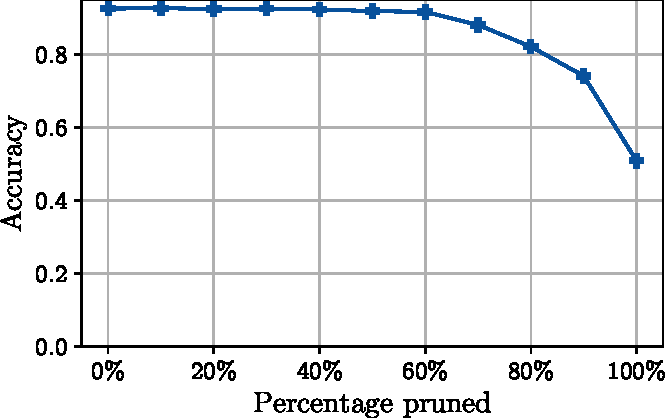
\includegraphics[width=\textwidth]{img/pruning_bert_sst.pdf}
\caption{\label{fig:incremental_pruning_sst} Evolution of accuracy on the validation set of \textbf{SST-2} when heads are pruned from \bertmnli{} according to $I_h$.}
\end{subfigure}
~
\begin{subfigure}[t]{0.48\textwidth}
\centering
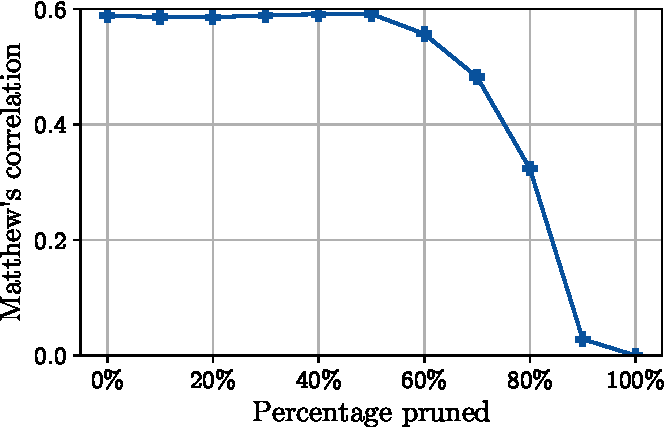
\includegraphics[width=\textwidth]{img/pruning_bert_cola.pdf}
\caption{\label{fig:incremental_pruning_cola} Evolution of Matthew's correlation on the validation set of \textbf{CoLA} when heads are pruned from \bertmnli{} according to $I_h$.}
\end{subfigure}
~
\begin{subfigure}[t]{0.48\textwidth}
\centering
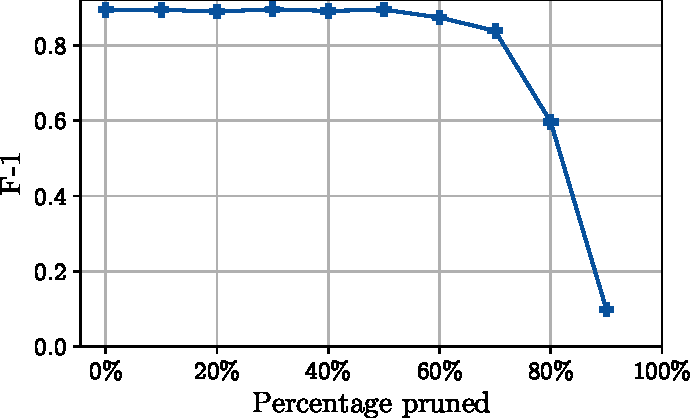
\includegraphics[width=\textwidth]{img/pruning_bert_mrpc.pdf}
\caption{\label{fig:incremental_pruning_mrpc} Evolution of F-1 score on the validation set of \textbf{MRPC} when heads are pruned from \bertmnli{} according to $I_h$.}
\end{subfigure}
~
\begin{subfigure}[t]{0.48\textwidth}
\centering
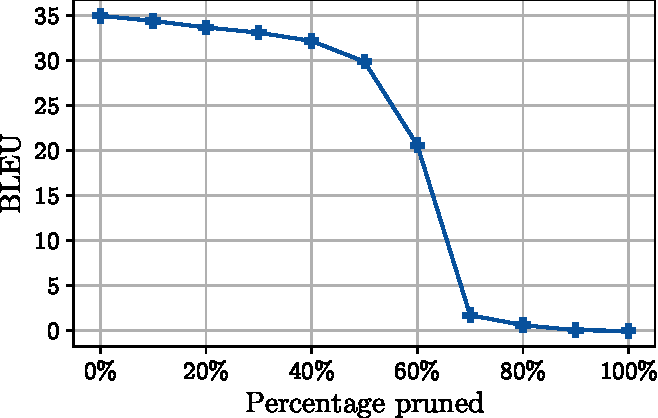
\includegraphics[width=\textwidth]{img/pruning_iwslt.pdf}
\caption{\label{fig:incremental_pruning_iwslt} Evolution of the BLEU score of our \textbf{IWSLT} model when heads are pruned according to $I_h$ (solid blue).}
\end{subfigure}
\caption{\label{fig:incremental_pruning_appendix}Evolution of score by percentage of heads pruned.}
\end{figure*}
